\section{Motion Extraction}
Motion can be the only cue for segmentation - camouflage is only visible in motion\\
\\
Some applications of motion extraction:
\begin{itemize}
	\item change / shot cut detection in films
	\item surveillance / traffic monitoring
	\item autonomous driving
	\item analyzing game dynamics in sports
	\item motion capture / gesture analysis
	\item image stabilisation
	\item motion compensation (e.g. medical robotics)
	\item feature tracking for 3D reconstruction (structure from motion)
\end{itemize}

\subsection{Optical Flow}
Optical Flow = apparent motion of brightness patterns\\
\\
Ideally, the optical flow is the projection of the threedimensional motion vectors on the image - Such 2D motion vector is sought at \textbf{every} pixel of the image (a motion vector here is a 2D translation vector)\\
\\
Suppose a point of the scene projects to a certain pixel of the current video frame. Our task is to figure out to which pixel in the next frame it moves…
In order to find these corresponding pixels, we need to come up with a reasonable assumption on how we can detect them among the many.
We assume these corresponding pixels have the same intensities as the pixels the scene points came from in the previous frame.\\
\\
Two examples where following brightness patterns is misleading:
\begin{enumerate}
	\item Untextured, rotating sphere $O.F. = 0$
	\item No motion, but changing lighting $O.F. \neq 0$
\end{enumerate}

\subsubsection{Mathematical formulation}
I (x,y,t) = brightness at (x,y) at time t - one equatio per pixel

$$
\frac{DI}{Dt} = \frac{\partial I}{\partial x}\frac{\partial x}{\partial t}+\frac{\partial I}{\partial y}\frac{\partial y}{\partial t}+\frac{\partial I}{\partial t} = I_x u + I_y v + I_t = 0
$$

The three derivates can be measured but the velocity u,v are unknown.

\textit{something calculus}



Horn \& Schunck algorithm

\textit{something solution of problem}

\begin{itemize}
	\item errors at object boundaries
	\item example of regularization
\end{itemize}

\subsection{Condensation Filter {\small or condensation tracker}}

System model (f = system transition function)
$$x_t = f_{t-1}(x_{t-1},w_{t-1}) $$
Measurement model (h = measurement function)
$$ z_t = h_t(x_t,v_t) $$
and $Z_t = (z_1, \dots , z_t)$ is the history of observations\\

\subsubsection{Recursive Bayesian filter (Kalman filter)}
Object not as a single state but a probabilistic distribution.\\
\\
1. prediction
$$
p(x_t | Z_{t-1}) = \int p(x_t | x_{t-1}) p(x_{t-1} | Z_{t-1}) dx_{t-1}
$$
2. measurement update
$$
p(x_t | Z_t) = \frac{p(Z_t | x_t) p(x_t | Z_{t-1})}{p(Z_t | Z_{t-1})}
$$

Problem integral is computational heavy to compute -> condensation tracker (particle filter)

\subsubsection{Particle Filter}
\begin{multicols}{2}
	1. prediction\\
	Start with $S_{t-1}$, the sample set of the previous step, and apply the system model to each sample, yielding predicted samples $s_t$.\\
	2. update\\
	Scale each particle by the measurement likelihood. Weight the particles.\\
	3. resample\\
	resample to get $N$ particles with equal weights.
	
	\columnbreak
	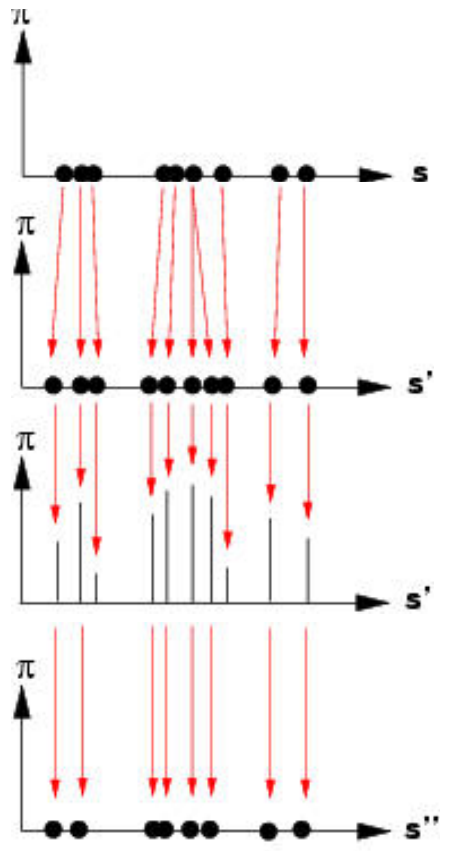
\includegraphics[width=0.7\columnwidth]{pictures/particlefilter}
\end{multicols}

In the limit (large N) equivalent to Bayesian tracker

\subsubsection{Comparison Particle Filter - Kalman filter}
{\footnotesize \begin{multicols}{2}
	\begin{itemize}
		\item Unrestricted system models
		\item Unrestricted noise models
		\item Multiple hypotheses
		\item Discretisation error
		\item Postprocessing for interpret
	\end{itemize}
	\columnbreak
	\begin{itemize}
		\item Linear system models
		\item Gaussian noise
		\item Unimodal
		\item Exact solution
		\item Direct interpretation
	\end{itemize}
\end{multicols}}
